\section{Diseño del pipeline del modelo propuesto de generación de árboles de comportamiento}
\label{sec:ModeloBT}

Antes de diseñar e implementar la herramienta se ha buscado tener claro el diseño de cuál debería ser el flujo de ejecución, así como los diferentes módulos que la iban a componer.

\begin{figure}[H]
    \centering
    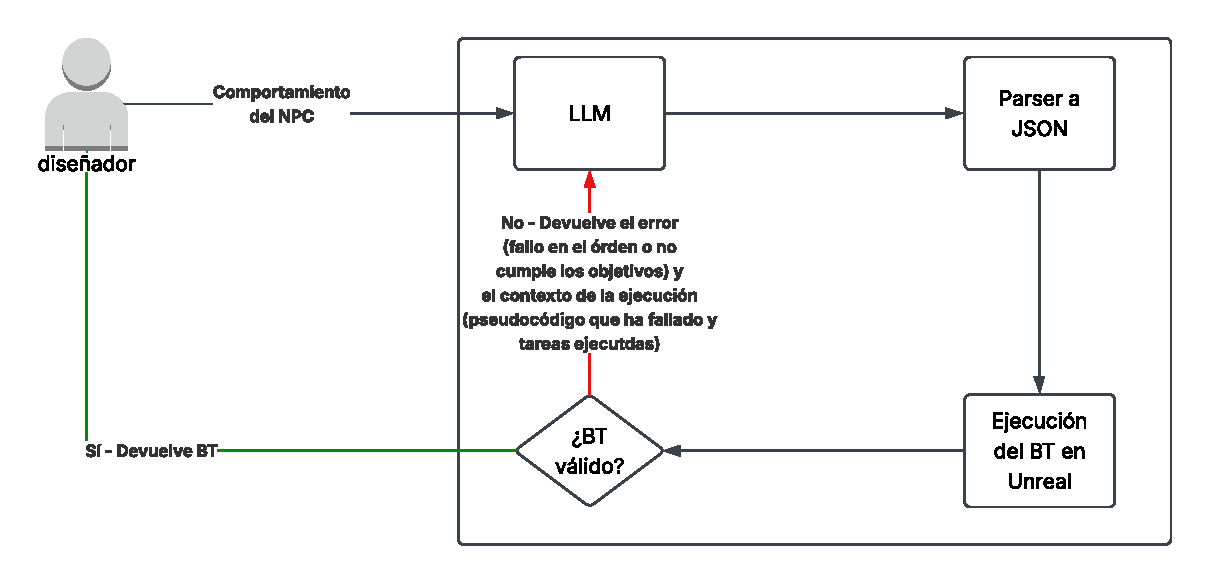
\includegraphics[width=1.0\textwidth]{Imagenes/Vectorial/DiagramaHerramienta.pdf}
    \caption[Diagrama de la herramienta propuesta]{Diagrama donde se visualiza el flujo de la herramienta propuesta.}
    \label{fig:diagramaHerramienta}
\end{figure}

En la figura \ref{fig:diagramaHerramienta} se puede ver el flujo de ejecución propuesto:

\begin{enumerate}
    \item El diseñador describe el comportamiento buscado para un NPC.
    \item Fuera del entorno del motor de videojuegos se genera el árbol de comportamiento mediante LLMs en un formato JSON.
    \item El motor de videojuegos traduce y crea el árbol de comportamiento generado.
    \item Se ejecuta el árbol.
    \item Opcionalmente se valida el árbol de forma automática. En caso de ser un árbol válido se termina la ejecución. En caso contrario se devuelve al modelo generador el árbol fallido y se le avisa del error.
\end{enumerate}

Este pipeline busca la independencia entre el motor de videojuegos y los modelos LLM, así como una opacidad de la generación frente a los usuarios y la simplicidad para diseñadores que no tengan un perfil muy técnico.

En las siguientes secciones de este capítulo se explicará el entorno de pruebas desarrollado para este trabajo, así como la implementación de la generación de los BTs, la validación de éstos y las pruebas a usuarios realizadas.